\lstset{language=bash}
\newpage
\chapter{Background}
% ==============================================================================
% \section{What is a Version Control System}
% A version Control System (VCS) saves modifications done by individual software developers, making the process more accessible since they can track their work over time. In addition, it helps share data between nodes where each node can be kept up to date with updated versions, so there is no need for any merge conflicts.
%
% The advantages provided by VCS include: aiding in collaboration among programmers, improved efficiency when working on larger groups of mixed products; providing an audit trail; easy branching functionality; simplifying team-based development; understanding who has worked on specific pieces or sections during what period in time but also making sure that all changes are appropriately tracked providing transparency within teams while maintaining optimal performance levels through streamlined management processes, helping avoid errors arising from inconsistency between versions such as mismatched documents or programming problems resulting from conflicting edit operations.
% \subsection{What is the purpose of Version Control Systems}
% For almost all software projects, the source code is an asset that must be protected. For most software teams, the source code is a repository of invaluable knowledge and understanding about the problem domain that developers have collected and refined through careful effort. Version control protects this priceless resource in many ways: it prevents catastrophe or casual degradation from occurring and prevents human error or unintended consequences from affecting its quality.
%
% For example, software developers working in teams continually write new source code and change existing code; these are organized into file folders called "file trees". One developer may be working on a new feature while another fixes an unrelated bug by changing parts of the file tree; each developer may change several parts at once.
%
% Version control can help teams solve these kinds of problems because every individual change made by each contributor is tracked, helping prevent concurrent work from conflicting with one another so that any incompatibility should be discovered and solved without blocking team members' progress further down the line (this will also ensure that any changes being made do not introduce bugs).
%
% Further still, testing for new versions cannot occur until some development work is done beforehand. This means both processes move forward together until they reach their newest version - thus decreasing risk to both sides due to errors along either path.
% \section{Types of VCS}
% The two approaches to VCSs are Centralized and Distributed. Both approaches are in widespread use today. The centralized approach is based on the client-server model, where a single central repository stores the history of all files. In contrast, the distributed approach provides each user with a full repository copy.
%
% While there is no clear answer for which approach is best, it's important to note that the centralized approach features a single point of failure but also more challenging scaling than its counterpart (Distributed).
%
% % \newpage
% \subsection{Centralized Version Control Systems (CVCS)}
% A centralized Version Control System is a system that enables developers to work together on the same project by storing the primary copy of files in a central repository. This system keeps track of all files and saves information in the local repository. CVCS are called centralized because there is only one central server or repository.
%
% The server maintains a complete record of issues, while clients only maintain a local copy of the shared documents. All developers make their modifications to the repository through checkout. However, only the last version of the files is retrieved from the server, meaning any modifications made will automatically be shared with other developers.
%
% Users can modify in parallel with their local copy of shared documents and sync with the central server to release their contributions and make them visible to other collaborators. However, because centralized version control systems rely on one repository that includes the correct project version, they must restrict write access so that only trusted contributors can commit modifications.
%
% CVCS has some challenges, such as if the central server is inaccessible, users will not be able to merge their work or save the released modifications. Also, if the central repository is corrupted, everything will be lost. Contributors must be the ones who have writing permissions to perform basic tasks, such as reverting modifications to a previous state, creating or merging branches, or releasing modifications with complete revision history. This limitation affects participation and authorship for new contributors.
%
% So, the main drawbacks of using CVCS are that it requires a network connection to work on the source code, developers must order to contribute to a project, and a single point of failure is an issue when using one server.
%
% \begin{figure}[htbp]
%     \centering
%     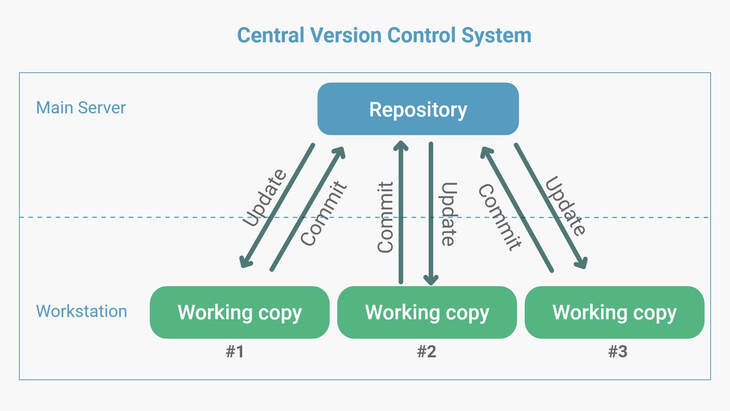
\includegraphics[width=0.75\textwidth]{centralized-vcs-structure}
%     \caption{Centralized Version Control System}
%     \label{fig:cvcs-structure}
% \end{figure}
%
% % \newpage
% \subsection{Distributed Version Control Systems (DVCS)}
% Distributed Version Control Systems (DVCS) were created to overcome the limitations of Centralized Version Control Systems (CVCS), which enable branching and merging, avoid local VCS operations and allow developer collaboration. Due to the limitations associated with using a centralized version control system, Open Source Software (OSS) projects today broadly adopt DVCS.
%
% DVCS is designed to work in two ways: it keeps file histories locally on each device. However, it can also sync local user modifications with servers again when necessary so that these modifications can be shared with everyone else. In addition, in DVCS, developers can work separately or together on the same project, as they have access to all repositories needed for their task; any repository can be cloned from another, so there is no repository more important than others.
%
% To provide a new way for versioning software artefacts, several Distributed Version Control Systems emerged in the software field, such as \lstinline{Mercurial}, \lstinline{Git}, \lstinline{Bazaar}, etc. These tools have been adopted by many Open Source Software (OSS). The operations in DVCS are much faster than those found in CVSS because they are done locally, while CVSS operations require remote connection; some consider that distributed systems will soon replace centralized ones because they suit more substantial projects with more independent developers who want full functionality even without network connection available, offer advantages like earlier drafts of your work being saved without requiring you releasing them publicly or sharing them with other people etc.
%
% Collaboration between team members and allowing individual developers to be servers or clients are the most important features of version control systems, so developers can work on source code without being connected to a central or remote repository.
%
% DVCS introduces some challenges: it lacks a coherent version numbering system, where there is no centralized versioning server, and uses hash modifications or a unique GUID. So, the lack of a central server makes system backup difficult.
%
% % \newpage
% The two most prevalent complaints about the disadvantages of DVCS are that: pessimistic locks are not available and they have weak tools for binary. However, the reasons for the transition from centralized to decentralized version Control Systems are that developers can work offline and work incrementally efficiently because they can make several roles, such as developing new tasks or fixing errors; this also leads to exploratory coding, which gives them more freedom in their workflow while still retaining control over their code's release schedule.
%
% \begin{figure}[htbp]
%     \centering
%     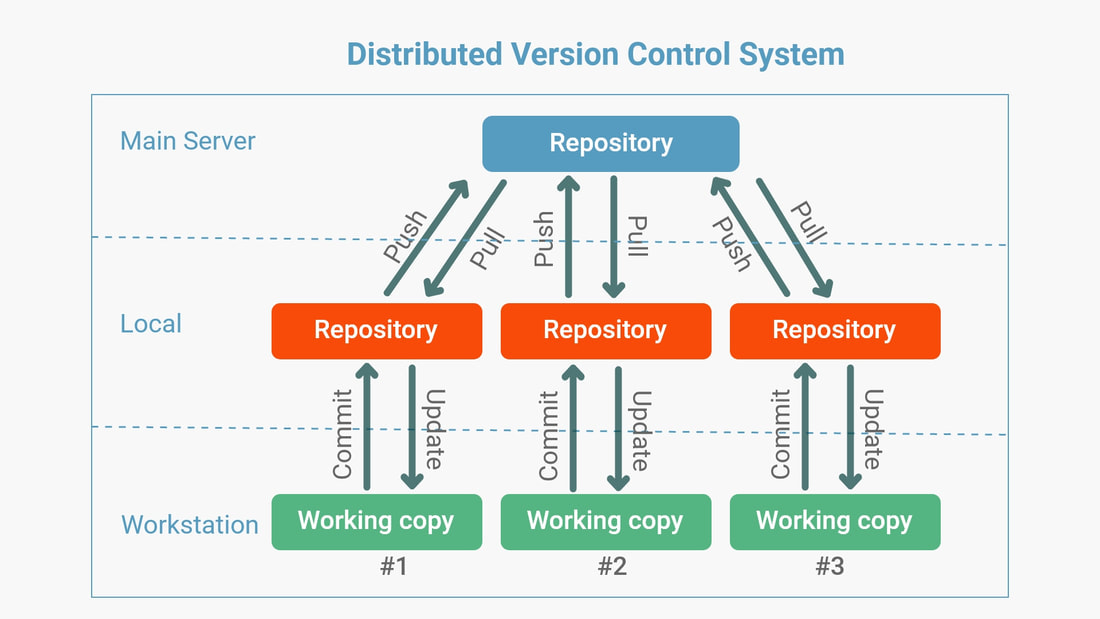
\includegraphics[width=0.8\textwidth]{distributed-vcs-structure}
%     \caption{Distributed Version Control System}
%     \label{fig:dvcs-structure}
% \end{figure}
%
% % \newpage
%
%
% ==============================================================================
%
% \section{What is a Version Control System}
% A Version Control System (VCS) saves modifications done by individual software developers, making the process more accessible since they can track their work over time. In addition, it helps share data between nodes where each node can be kept up to date with updated versions, so there is usually no need to handle merge conflicts.
%
% The advantages provided by VCS include: aiding in collaboration among programmers, improved efficiency when working on larger groups of mixed products; providing an audit trail; easy branching functionality; simplifying team-based development; understanding who has worked on specific pieces or sections during what period in time but also making sure that all changes are appropriately tracked providing transparency within teams while maintaining optimal performance levels through streamlined management processes, helping avoid errors arising from inconsistency between versions such as mismatched documents or programming problems resulting from conflicting edit operations.
% \paragraph{What is the purpose of Version Control Systems?}
% \hfill\medskip\\
% For almost all software projects, the source code is an asset that must be protected. Moreover, for most software teams, the source code is a repository of invaluable knowledge and understanding about the problem that developers have collected and refined through careful effort.
%
% Version control protects this priceless resource in many ways: it prevents catastrophe or casual degradation from occurring and prevents human error or unintended consequences from affecting its quality.
%
% For example, software developers working in teams continually write new source code and change existing code; these are organized into file folders called "file trees". One developer may work on a new feature while another fixes an unrelated bug by changing parts of the file tree; each developer may change several parts simultaneously.
%
% Version control can help teams solve these kinds of problems because every individual change made by each contributor is tracked, helping prevent concurrent work from conflicting with one another so that any incompatibility should be discovered and solved without blocking team members' progress further down the line (this will also ensure that any changes being made do not introduce bugs).
%
% Further still, testing for new versions cannot occur until some development work is done beforehand. This means both processes move forward together until they reach their newest version - thus decreasing risk to both sides due to errors along either path.
%
% ==============================================================================
%
% \section{What is a Version Control System}
\section{What is a Version Control System}
A \acrfull{vcs} saves modifications made by individual software developers, allowing them to track their work over time and making the process more accessible. Furthermore, it facilitates sharing data between nodes, where each node can be kept up to date with the latest versions, minimising the need to handle merge conflicts.
\smallskip

\acrlongpl{vcs} provide several advantages, such as aiding in collaboration among programmers and improving efficiency when working on large groups of mixed products. In addition, \acrshortpl{vcs} offer an audit trail and easy branching functionality, simplifying team-based development. It also enables an understanding of who has worked on specific pieces or sections during a given period.
\smallskip

By ensuring all changes are appropriately tracked, \acrshortpl{vcs} promote transparency within teams while maintaining optimal performance levels through streamlined management processes. This helps avoid errors arising from inconsistencies between versions, such as mismatched documents or programming problems resulting from conflicting edit operations.

\paragraph{Significance of Version Control Systems}
\hfill\medskip\\
For most software projects, the source code is a valuable asset that must be protected. Additionally, for many software teams, the source code represents a repository of invaluable knowledge and understanding about the problem that developers have amassed and refined through meticulous effort.
\smallskip

Version control safeguards this precious resource by preventing catastrophes, casual degradation, human error, or unintended consequences from affecting its quality. Software developers working in teams continually write new source code and modify existing code, which is organised into file folders called "file trees". Developers may work on different tasks simultaneously, such as implementing new features or fixing unrelated bugs, by altering parts of the file tree.
\smallskip

Version control assists teams in addressing these challenges by tracking each change made by contributors, helping to prevent concurrent work from conflicting with one another. Consequently, any incompatibility can be detected and resolved without impeding team members' progress further down the line, ensuring that changes do not introduce bugs.

% \section{Existing Version Control Systems}
\section{Evolution of Version Control Systems}
\begin{figure}[htbp]
    \centering
    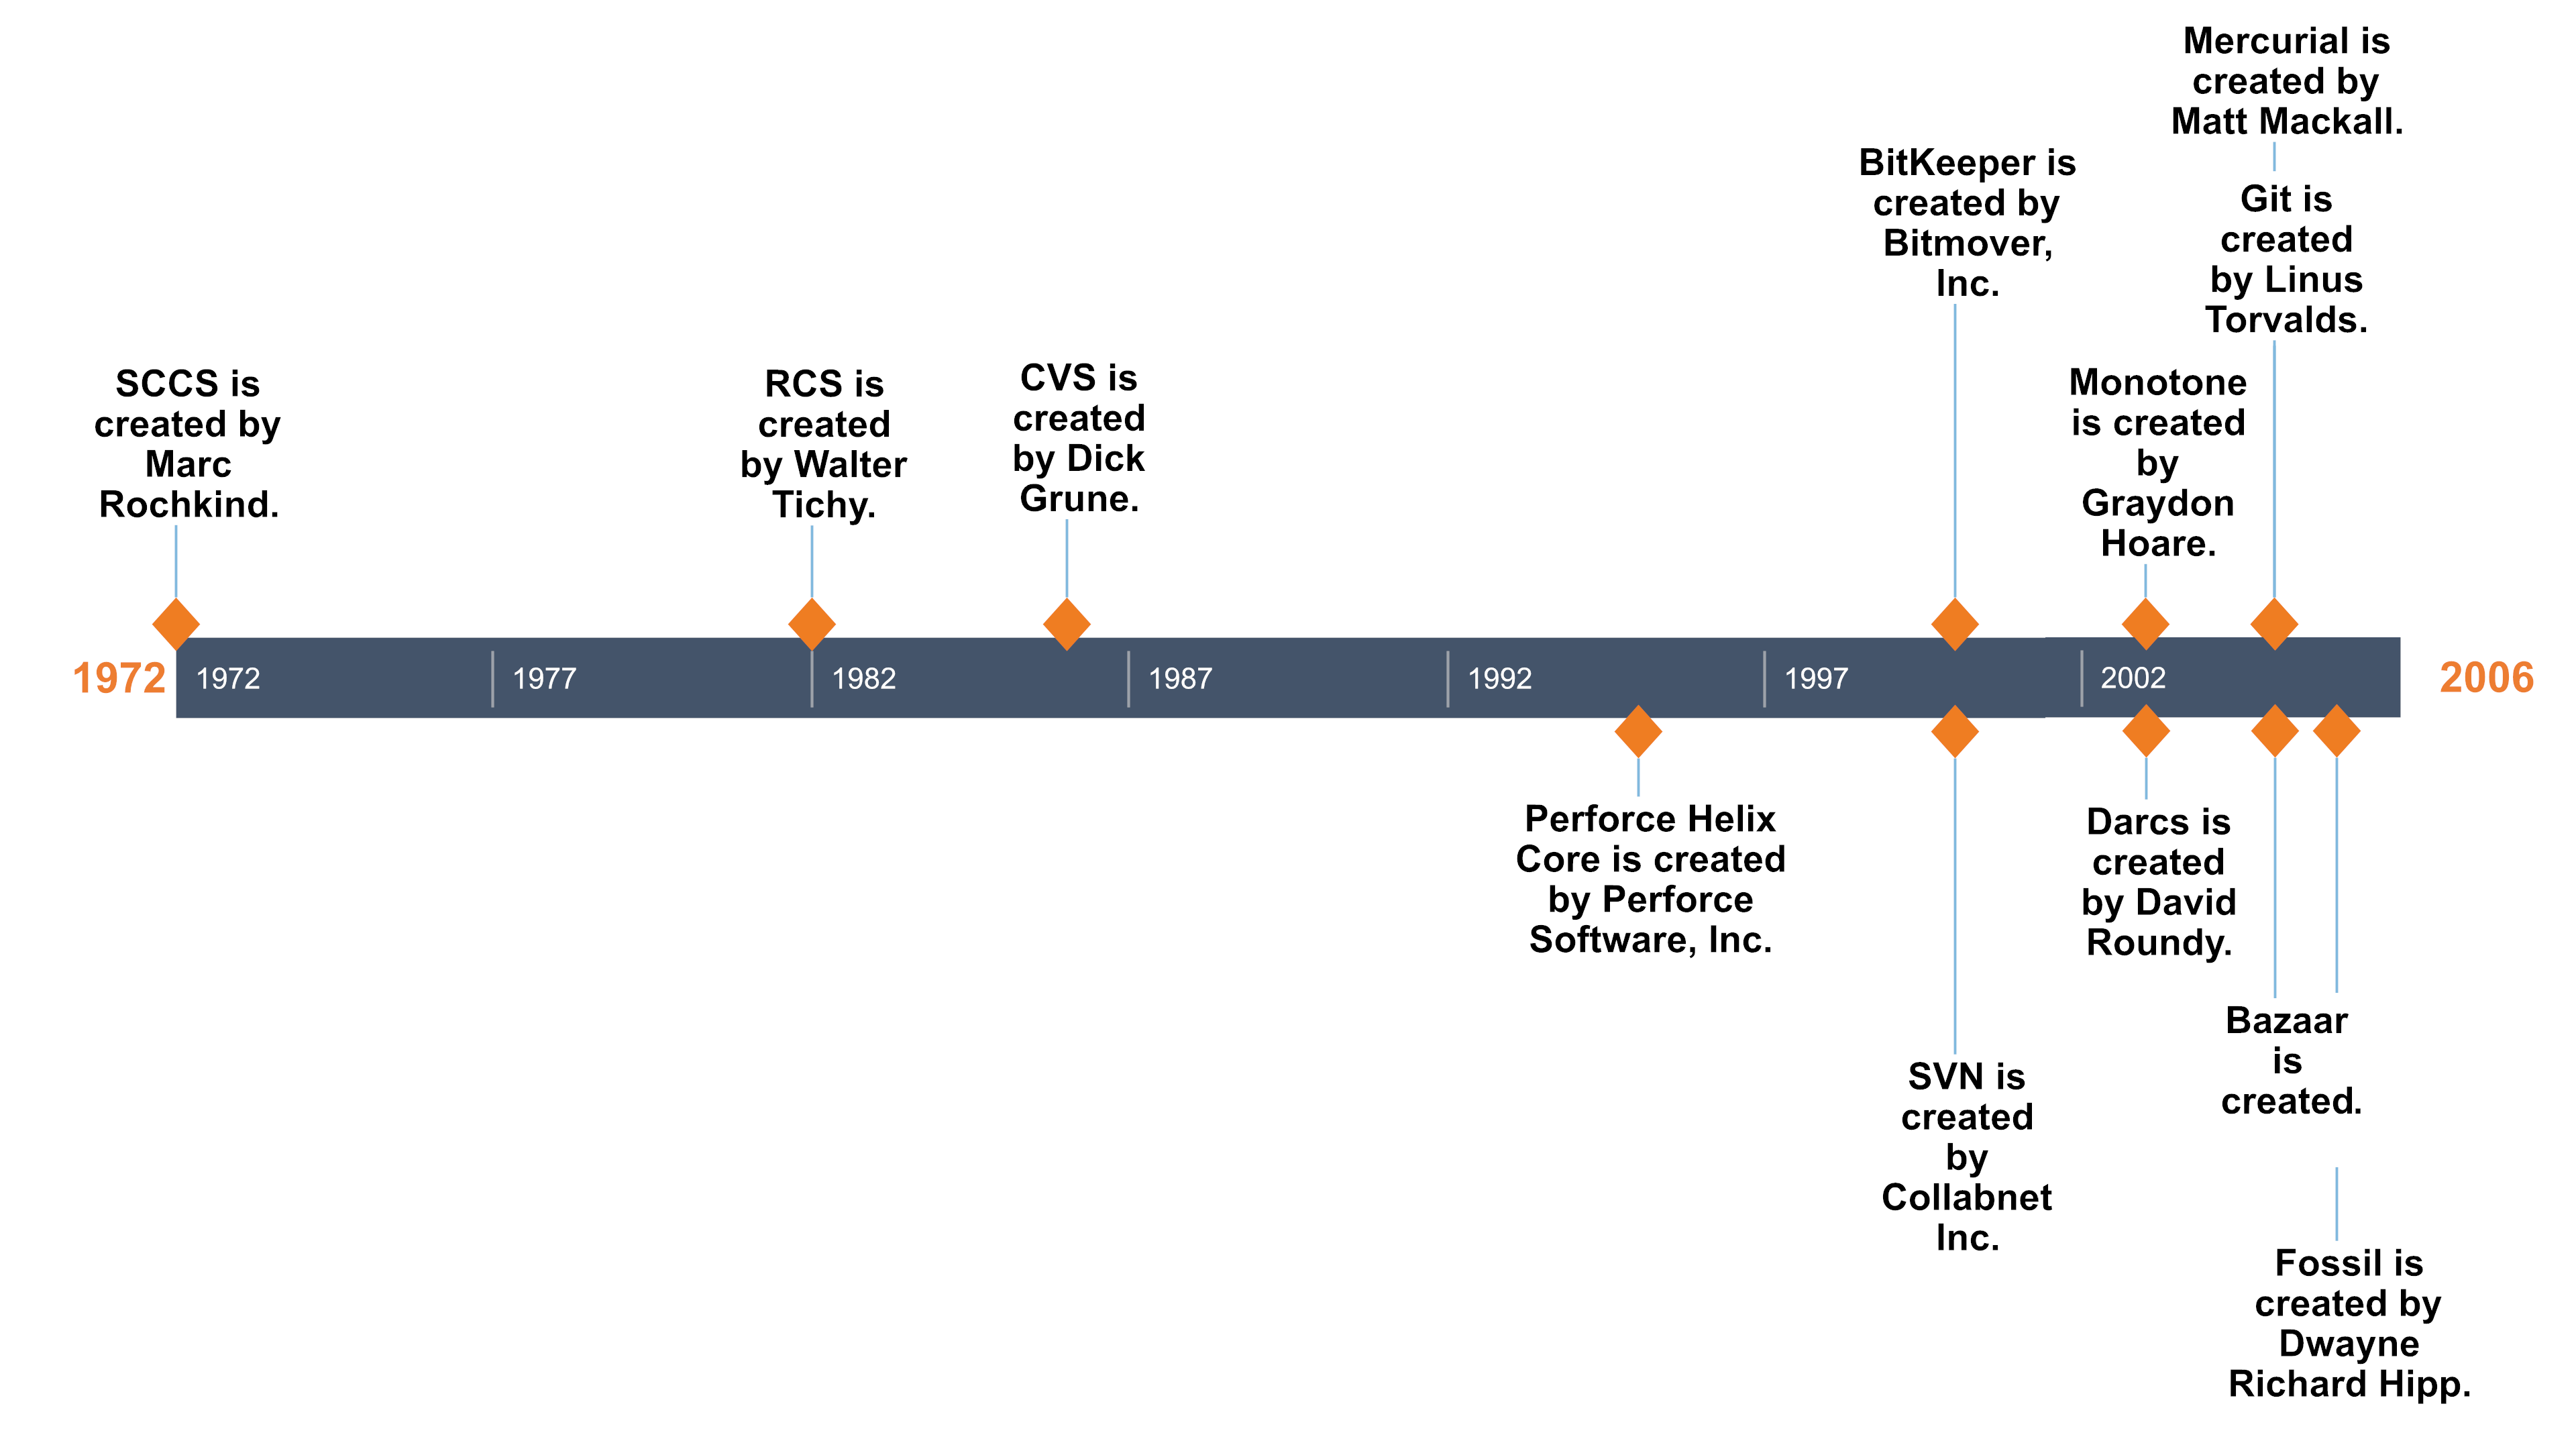
\includegraphics[width=0.95\textwidth]{vcs-timeline.png}
    \caption{Timeline of the Creation of Version Control Systems \cite{stopak_2019}}
    \label{fig:vcs-timeline}
\end{figure}
\subsection{Local Version Control Systems (LVCS)}
% Early VCS were intended to track changes for individual files and checked-out files could only be edited locally by one user at a time. They were built on the assumption that all users would log into the same shared Unix host with their own accounts, but it was not always possible. As you can imagine, these early systems made it easier for small teams to revisit code states from various points in history.
Local Version Control Systems are systems designed to operate on a single machine, early VCSs were intended to track changes for individual files, and checked-out files could only be edited locally by one user at a time. In addition, they were built on the assumption that all users would log into the same shared Unix host with their own accounts, which was not always possible.
\smallskip

The main benefit of LVCS is that it provides a basic level of version control functionality without requiring any network connectivity. However, this can also be seen as a drawback when you consider that with LVCS, there is no central repository to store the code, which means that each developer has their own copy. This can lead to issues with merging changes and tracking changes across multiple copies.

\begin{figure}[htbp]
    \centering
    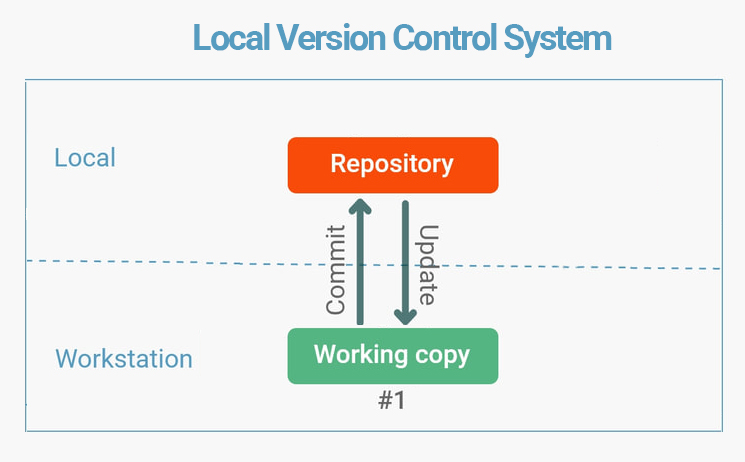
\includegraphics[width=0.8\textwidth]{local-vcs-structure}
    \caption{Local Version Control System (LVCS)}
    \label{fig:lvcs-structure}
\end{figure}

% \subsubsection{Source Code Control System (SCCS)}
\subsubsection{\texorpdfstring{\acrfull*{sccs}}{Source Code Control System (SCCS)}}
\label{sec:sccs}
% SCCS was released in 1972 and is one of the first successful VCS tools. It was written by Marc Rochkind at Bell Labs, who wanted to solve the problem of tracking file revisions. The tool made tracking down bugs introduced into a program significantly more manageable. SCCS is worth understanding at a basic level because it helped set up modern VCS tools that developers use today.
\acrlong{sccs} was released in 1972 and is one of the first successful \acrshort{vcs} tools \cite{stopak_2019}. It was written by Marc Rochkind at Bell Labs, who wanted to solve the problem of tracking file revisions. The tool made tracking down bugs introduced into a program significantly more manageable. \acrshort{sccs} is worth understanding at a basic level because it helped set up modern \acrshort{vcs} tools that developers use today.
\paragraph{Architecture}
% Much like modern VCS tools, SCCS has a set of commands that allow developers to work with versioning of files. The basic command functionality are:
Much like modern \acrshort{vcs} tools, \acrshort{sccs} has a set of commands that allow developers to work with the versioning of files. The basic command functionality is:
\begin{itemize}
    \item Check-in files to track their history.
    \item Check-out specific file versions for review.
    \item Check-out specific file versions for editing.
    \item Check-in new file versions with comments explaining the changes.
    \item Revert changes made to a checked-out file.
    \item Basic branching and merging of changes.
    \item Print a log of a file's version history.
\end{itemize}
% A special type of file called a \lstinline{s-file} or a \lstinline{history file} is created when a file is tracked by SCCS. This file is named with the original filename prefixed with a \lstinline{s.}, and is stored in a subdirectory called \lstinline{SCCS}.
A particular type of file called an \lstinline{s-file} or a \lstinline{history file} is created when a file is tracked by SCCS. This file is named with the original filename prefixed with an \lstinline{s.} and is stored in a subdirectory called \lstinline{SCCS}.
\smallskip

So a file called \lstinline{test.txt} would get a history file created in the \lstinline{./SCCS/} directory with the name of \lstinline{s.test.txt}. When created, the \lstinline{s-file} contains the original file contents, a header that contains the file's version number, and some other metadata. There are also checksums stored in the \lstinline{s-file} that are used to verify the integrity of the file (i.e. to ensure that the file has not been tampered with). The \lstinline{s-file} content is not encoded or compressed in any way, which is a clear difference from modern VCS tools.
\smallskip

Since the original file's content is now stored in the history file, it can be retrieved into the working directory for review, compilation, or editing. Further changes made to this new copy, such as line additions, modifications and removals, can be checked back into a revised version of the history file, which increments its revision number \cite{stopak_2019}.
\smallskip

Subsequent SCCS check-ins only store only deltas or changes to a file instead of storing entire contents each time; when a check-in is made, subsequent revisions are added onto existing delta tables inside an amended history file (history files do not use compression). This decreases the size of these large histories since they are not using compression on their files, so they take up more space than just having one complete copy that you are tracking with no differences like Word docs etc.
\smallskip

As previously mentioned, SCCS uses the Delta method known as Interleaved Deltas, which allows constant-time checkout regardless of how old your checked-out revision is - i.e., older revisions do not take longer than newer ones.
\smallskip

It is important to note that all files are tracked and checked in separately; there is no way to check in changes on multiple files as a part of one atomic unit - like a commit in \nameref{sec:git}. Each tracked file has its corresponding history file, which stores revisions. Generally, this means that the version numbers of different files cannot match each other. However, matching revision numbers can be achieved by editing every file at once (even if not all of the changed areas have fundamental changes) and checking them all together. This will increment revision numbers for any modified content, so they will be consistent with their revisions—but it's not comparable to including lots of different pieces within a single commit like you would in \nameref{sec:git}. In SCCS, these make individual check-ins across separate history folders rather than one extensive report containing everything at once.
\smallskip

When a file is checked out for editing in SCCS, it is locked so that anyone else cannot edit it. This prevents changes from being overwritten by other users and limits development since only one user can edit the file simultaneously.
\smallskip

The software supports branches that store sequences of changes to specific files - these can then be merged back into the original versions or with copies of other branched versions of the same parent branch.

\paragraph{Basic Commands}

\begin{itemize}
    \item \lstinline{sccs create <filename.ext>} - Check in a new file to SCCS and create a new history file for it (in the \lstinline{./SCCS/} directory by default).
    \item \lstinline{sccs get <filename.ext>} - Check out a file from from its corresponding history file and place it in the working directory in readonly mode.
    \item \lstinline{sccs edit <filename.ext>} - Check out a file from the corresponding history file for editing. Locks the history file so no other users can modify it.
    \item \lstinline{sccs delta <filename.ext>} - Check in the modifications to the specified file. Will prompt for a comment, store the changes in the history file, and remove the lock.
    \item \lstinline{sccs prt <filename.ext>} - Display the revision log for a tracked file.
    \item \lstinline{sccs diffs <filename.ext>} - Display the differences between the current working copy of a file and the state of the file when it was checked out.
\end{itemize}

\subsubsection{Revision Control System (RCS)}
% TODO: Explain RCS
The Revision Control System (RCS) was released in 1982; it was written in C by Walter Tichy as an alternative to SCCS, which was still closed-source at the time. RCS was released under the GNU General Public License, which allowed it to be used in open-source projects.

\begin{quote}
    "RCS manages revisions of text documents, in particular source programs, documentation, and test data. It automates the storing, retrieval, logging and identification of revisions." -- Walter Tichy \cite{tichy_1985}
\end{quote}

\paragraph{Architecture}
RCS shares many traits with its predecessor, including:
\begin{itemize}
    \item Handling revisions on a file-by-file basis.
    \item Changes across multiple files can't be grouped together into an atomic commit.
    \item Tracked files are intended to be modified by one user at a time.
    \item No network functionality.
    \item Revisions for each tracked file are stored in a corresponding history file.
    \item Basic branching and merging of revisions within individual files.
\end{itemize}
When a file is set checked into RCS for the first time, a corresponding history file is created for it in the local \lstinline{./RCS/} directory. This file is postfixed with a \lstinline{,v} so a file named \lstinline{test.txt} would be tracked by a file called \lstinline{test.txt,v}.

RCS uses a \lstinline{reverse-delta} scheme for storing file changes. When a file is checked in, the history file contains the complete snapshot of its contents. When that same file is modified and checked in again, RCS calculates only one delta--the difference between the new version of that particular revision and the old version as recorded previously by RCS--and saves it along with an older snapshot if necessary.

This is called \lstinline{reverse-delta} because to check out an earlier revision, RCS starts from what is newest and applies consecutive deltas until getting back to our desired revision; starting at what is newest allows for quick checkout times since we always have access to current revisions (since their snapshots are saved).

However, suppose you wanted to go back further than just one recent update on your project (1 or 2 old versions). In that case, things get considerably more complicated because those versions' snapshots would need to be calculated against each other before they can be applied to what is new.

This is not the case with SCCS since it takes the same amount of time to fetch any revision. In addition, no checksum is stored in RCS history files; therefore, file integrity cannot be ensured.

% TODO: List RCS commands
\paragraph{Basic Commands}

\begin{itemize}
    \item \lstinline{ci <filename.ext>} - Check in a new file to RCS and create a new history file for it (in the \lstinline{./RCS/} directory by default).
    \item \lstinline{co <filename.ext>} - Check out a file from from its corresponding history file and place it in the working directory in readonly mode.
    \item \lstinline{co -l <filename.ext>} - Check out a file from the corresponding history file for editing. Locks the history file so no other users can modify it.
    \item \lstinline{ci <filename.ext>} - Check in file changes and create a new revision for it in its corresponding history file.
    \item \lstinline{merge <file-to-merge-into.ext> <parent.ext> <file-to-merge-from.ext>} - Merge changes from two modified children of the same parent file.
    \item \lstinline{rcsdiff <filename.ext>} - Display the differences between the current working copy of a file and the state of the file when it was checked out.
    \item \lstinline{rcsclean} - Removes working files that don't have locks on them.
\end{itemize}

\subsection{Centralized Version Control Systems (CVCS)}
% Version control technology continued to evolve, leading to centralized repositories that contained the 'official' versions of their projects. This was good progress since it allowed multiple users to checkout, work with the code simultaneously, and commit to this central repository. Furthermore, network access was required for people who wanted to commit changes they had made locally.
A centralized Version Control System is a system that enables developers to work together on the same project by storing the primary copy of files in a central repository. This system keeps track of all files and saves information in the local repository. CVCS are called centralized because there is only one central server or repository.

The server maintains a complete record of issues, while clients only maintain a local copy of the shared documents. All developers make their modifications to the repository through checkout. However, only the last version of the files is retrieved from the server, meaning any modifications made will automatically be shared with other developers.

Users can modify in parallel with their local copy of shared documents and sync with the central server to release their contributions and make them visible to other collaborators. However, because centralized version control systems rely on one repository that includes the correct project version, they must restrict write access so that only trusted contributors can commit modifications.

CVCS has some challenges, such as if the central server is inaccessible, users will not be able to merge their work or save the released modifications. Also, if the central repository is corrupted, everything will be lost. Contributors must be the ones who have writing permissions to perform basic tasks, such as reverting modifications to a previous state, creating or merging branches, or releasing modifications with complete revision history. This limitation affects participation and authorship for new contributors.

So, the main drawbacks of using CVCS are that it requires a network connection to work on the source code, developers must order to contribute to a project, and a single point of failure is an issue when using one server.

\begin{figure}[htbp]
    \centering
    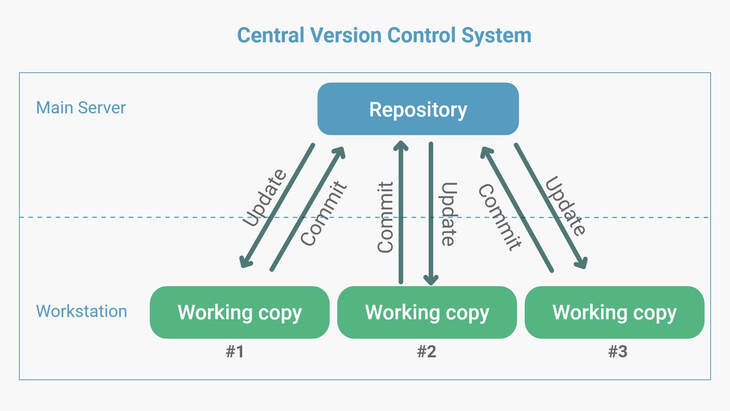
\includegraphics[width=0.85\textwidth]{centralized-vcs-structure}
    \caption{Centralized Version Control System (CVCS)}
    \label{fig:cvcs-structure}
\end{figure}

\subsubsection{Concurrent Versions System (CVS)}
Dick Grune developed the Concurrent Versions System in 1986. It was written in C, and its goal was to add a networking element to version control. As a result, the Concurrent Versions System became the first widely used VCS tool that allowed multiple users to work on the same project simultaneously from different locations. This kicked off the second generation of VCS tools, allowing geographically dispersed development teams to work together on a project.

\paragraph{Architecture}
CVS operates as a frontend for RCS - it provides a set of commands to interact with files in a project but uses the RCS history file format and commands behind the scenes.

This meant multiple developers could check out and work on the duplicate files for the first time in history. It did this by utilizing a centralized repository model.

The first step is to set up a centralized repository on a remote server using CVS. Projects can then be imported into the repository. When a project is imported into CVS, each file is converted into a \lstinline{,v} history file and stored in a central directory known as a \lstinline{module}. The repository generally lives on a remote server which is accessible over a local network or the Internet.

A developer checks out a copy of the module, which is copied to a working directory on their local machine. No files are locked in this process, so there is no limit to the number of developers that can check out the module at one time. Developers can modify their checked-out files and commit their changes as needed. If a developer commits a change, other developers need to update their working copies via a (usually) automated merge process before committing their changes. Occasionally merge conflicts will need to be manually resolved before the commit can be made. CVS also provides the ability to create and merge branches.

% TODO: List CVS commands
\paragraph{Basic Commands}

\begin{itemize}
    \item \lstinline{export CVSROOT=<path/to/repository>} - Sets the CVS repository root directory so it doesn't need to be specified in each command.
    \item \lstinline{cvs import -m 'Import module' <module-name> <vendor-tag> <release-tag>} - Import a directory of files into a CVS module. Before running this browse into the root directory of the project you want to import.
    \item \lstinline{cvs checkout <module-name>} - Copy a module to the working directory.
    \item \lstinline{cvs commit <filename.ext>} - Commit a changed file back to the module in the central repository.
    \item \lstinline{cvs add <filename.txt>} - Add a new file to track revisions for.
    \item \lstinline{cvs update} - Update the working copy by merging in committed changes that exist in the central repository but not the working copy.
    \item \lstinline{cvs status} - Show general information about the checked out working copy of a module.
    \item \lstinline{cvs tag <tag-name> <files>} - Add an identifying tag to a single file or set of files.
    \item \lstinline{cvs tag -b <new-branch-name>} - Create a new branch in the repository (must be checked out before working on it locally).
    \item \lstinline{cvs checkout -r <branch-name>} - Checkout an existing branch to the working directory.
    \item \lstinline{cvs update -j <branch-to-merge>} - Merge an existing branch into the local working copy.
\end{itemize}

\subsubsection{Apache Subversion (SVN)}
Subversion (SVN) was developed by CollabNet in 2000 and is now maintained by the Apache Software Foundation. It is written in C and was designed to be a more robust centralized solution than CVS.
\paragraph{Architecture}
% Similar to CVS, SVN uses a centralized repository model. Remote users must have a working network connection to commit their changes to the central repository.

% Subversion introduced the functionality of atomic commits which ensured that a commit would either fully succeed, or be completely abandoned if an issue occurred.

SVN, like CVS, uses a centralized repository model. Therefore, remote users must have a working network connection to commit their changes to the central repository.

Subversion introduced atomic commits, which ensure that a commit will either fully succeed or be completely abandoned if an issue occurs.

% In CVS, if a commit operation failed midway, for example due to a network outage, the repository could be left in a corrupted and inconsistent state. Furthermore, a commit or revision in Subversion can include multiple files and directories. This is important since it allows users to track sets of related changes together as a grouped unit, instead of the past storage models that track changes separately for each file.

If a commit operation in CVS fails, for example, due to a network outage, the repository can be corrupted and inconsistent. In Subversion, a commit or revision can include multiple files and directories. This allows users to track sets of related changes together as a grouped unit instead of separately for each file, like in past storage models.

% TODO: Rewrite this section
% ==============================================================================
The current storage model that Subversion uses for tracked files is called \lstinline{FSFS} or \lstinline{File System atop the File System}. This name was chosen since it creates its database structure using a file and directory structure that match the operating system filesystem it is running on. The unique feature of the Subversion filesystem is that it is designed to track not only the files and the directories it contains, but the different versions of these files and directories and they change over time. It is a filesystem with an added time dimension. In addition, folders are first class citizens in Subversion. Empty folders can be committed in Subversion, whereas in the rest (even Git) empty folders are unnoticed.

When a Subversion repository is created, a (nearly) empty database of files and folders is created as a part of it. A directory called \lstinline{db/revs} is created in which all revision tracking information for the checked-in (committed) files is stored. Each commit (which can include changes to multiple files) is stored in a new file in the \lstinline{revs} directory and is named with a sequential numeric identifier starting with 1. When a file is committed for the first time, its full content is stored. Future commits of the same file will store only the changes - also called the \lstinline{diffs} or \lstinline{deltas} - in order to conserve space. In addition, the deltas are compressed using \lstinline{lz4} or \lstinline{zlib} compression algorithms to further reduce their size.

By default, this is actually only true to a point. Although storing file deltas instead of the whole file each time does save on storage space, it adds time to checkout and commit operations since all the deltas need to be strung together in order to recreate the current state of the file. For this reason, by default Subversion stores up to 1023 deltas per file before storing a new full copy of the file. This achieves a nice balance of both storage and speed.

SVN does not use a conventional branching and tagging system. A normal Subversion repository layout is to have three folders in the root:
\begin{itemize}
    \item \lstinline{trunk/}
    \item \lstinline{branches/}
    \item \lstinline{tags/}
\end{itemize}
The \lstinline{trunk/} folder is used for the production version of the application.
The \lstinline{branches/} folder is used to store subfolders that correspond to individual branches.
The \lstinline{tags/} folder is used to store tags which represent specific (usually significant) project revisions.
% ==============================================================================

% TODO: List SVN commands
\paragraph{Basic Commands}
\begin{itemize}
    \item \lstinline{svn create <path-to-repository>} - Create a new, empty repository shell in the specified directory.
    \item \lstinline{svn import <path-to-project> <svn-url>} - Import a directory of files into the specified Subversion repository path.
    \item \lstinline{svn checkout <svn-path> <path-to-checkout>} - Copy a stored repository path to the desired working directory.
    \item \lstinline{svn commit -m 'Commit message'} - Commit a set of changed files and folders along with a descriptive commit message. These can be used as notes for future developers to understand what changes were made. The message of the initial commit is typically set to 'Initial commit'.
    \item \lstinline{svn add <filename.txt>} - Add a new file to track revisions for.
    \item \lstinline{svn update} - Update the working copy by merging in committed changes that exist in the central repository but not the working copy.
    \item \lstinline{svn status} - Show a list of tracked files that have been changed in the working directory (if any).
    \item \lstinline{svn info} - Show a list of general details about the checked-out copy.
    \item \lstinline{svn copy <branch-to-copy> <new-branch-path-and-name>} - Create a new branch by copying an existing one.
    \item \lstinline{svn switch <existing-branch>} - Switch the working directory to an existing branch. This will checkout the specified branch.
    \item \lstinline{svn merge <existing-branch>} - Merge the specified branch into the current branch checked out in the working directory. Note this needs to be committed afterwards.
    \item \lstinline{svn log} - Show the commit history and associated descriptive messages for the active branch (useful for devs to find details of previous changes).
\end{itemize}

% ==============================================================================
\subsubsection{Perforce Helix Core}
% Perforce is a centralized VCS that was developed by Perforce Software in 1995. Perforce is a commercial VCS that is used by many large companies, such as Google, Adobe and IBM. It is still one of the largest version control systems in use today.
% TODO: Rewrite this section
% ==============================================================================
Perforce Helix Core is a proprietary VCS created, owned, and maintained by Perforce Software, Inc. It is typically set up using a centralized model although it does offer a distributed model option. It is written in C and C++, and was initially released in 1995. It is primarily used by large companies that track and store a lot of content using large binary files, as is the case in the video game development industry. Although Helix Core is typically cost prohibitive for smaller projects, Perforce offers a free version for teams of up to 5 developers.
\paragraph{Architecture}
Perforce Helix Core is set up as a server/client model. The server is a process called \lstinline{p4d} which waits and listens for incoming client connections on a designated port, typically port 1666. The client is a process called \lstinline{p4} which comes in both command-line and GUI flavors. Users run the \lstinline{p4} client to connect to the server and issue commands to it. Support is available for various programming language APIs, including Python and Java. This allows automated issuance and processing of Helix Core commands via scripts. Integrations are also available for IDEs like Eclipse and Visual Studio, allowing users to work with version control from within those tools.

The Helix Core Server manages repositories referred to as depots, which store files in directory trees, not unlike Subversion (SVN). Clients can checkout sets of files and directories from the depots into local copies called \textbf{workspaces}. The atomic unit used to group and track changes in Helix Core depots is called the \textbf{changelist}. Changelists are similar to Git commits. Helix Core implements two similar forms of branching - \textbf{branches} and \textbf{streams}. Branches are conceptually similar to what we are used to - separate lines of development history. A stream is a branch with added functionality that Helix Core uses to provide recommendations on best merging practices throughout the development process.

When a file is added for tracking, Helix Core classifies it using a \textbf{file type} label. The two most commonly used file types are text and binary. For binary files, the entire file content is stored each time the file is stored. This is a common VCS tactic for dealing with binary files which are not amenable to the normal merge process, since manual conflict resolution is usually not possible.

For text files, only the deltas (changes between revisions) are stored. Text file history and deltas are stored using the RCS (Revision Control System) format, which tracks each file in a corresponding \lstinline{,v} file in the server depot. This is similar to CVS, which also leverages RCS file formats for preserving revision history. Files are often compressed using gzip when added to the depot and decompressed when synced back to the workspace.

% TODO: Add annotated comment
% It is suprising that such a longstanding proprietary software like Perforce would base itself on a seemingly antiquated and open-source root like RCS, especially for such an essential component (its delta and history file backend)...

% TODO: List Perforce commands
\paragraph{Basic Commands}

Below is a list of the most common Perforce commands.

% ==============================================================================
\subsection{Distributed Version Control Systems}
% In a distributed version control system, all copies of the repository are created equal - there is no central copy of the repository. This design principle encourages commits, branches and merges to be created locally without network access and pushed to other repositories as needed.
Distributed Version Control Systems (DVCS) were created to overcome the limitations of Centralized Version Control Systems (CVCS), which enable branching and merging, avoid local VCS operations and allow developer collaboration. Due to the limitations associated with using a centralized version control system, Open Source Software (OSS) projects today broadly adopt DVCS.

DVCS is designed to work in two ways: it keeps file histories locally on each device. However, it can also sync local user modifications with servers again when necessary so that these modifications can be shared with everyone else. In addition, in DVCS, developers can work separately or together on the same project, as they have access to all repositories needed for their task; any repository can be cloned from another, so there is no repository more important than others.

To provide a new way for versioning software artefacts, several Distributed Version Control Systems emerged in the software field, such as \lstinline{Mercurial}, \lstinline{Git}, \lstinline{Bazaar}, etc. These tools have been adopted by many Open Source Software (OSS). The operations in DVCS are much faster than those found in CVSS because they are done locally, while CVSS operations require remote connection; some consider that distributed systems will soon replace centralized ones because they suit more substantial projects with more independent developers who want full functionality even without network connection available, offer advantages like earlier drafts of your work being saved without requiring you releasing them publicly or sharing them with other people etc.

Collaboration between team members and allowing individual developers to be servers or clients are the most important features of version control systems, so developers can work on source code without being connected to a central or remote repository.

DVCS introduces some challenges: it lacks a coherent version numbering system, where there is no centralized versioning server, and uses hash modifications or a unique GUID. So, the lack of a central server makes system backup difficult.

% \newpage
The two most prevalent complaints about the disadvantages of DVCS are that: pessimistic locks are not available and they have weak tools for binary. However, the reasons for the transition from centralized to decentralized version Control Systems are that developers can work offline and work incrementally efficiently because they can make several roles, such as developing new tasks or fixing errors; this also leads to exploratory coding, which gives them more freedom in their workflow while still retaining control over their code's release schedule.

\begin{figure}[htbp]
    \centering
    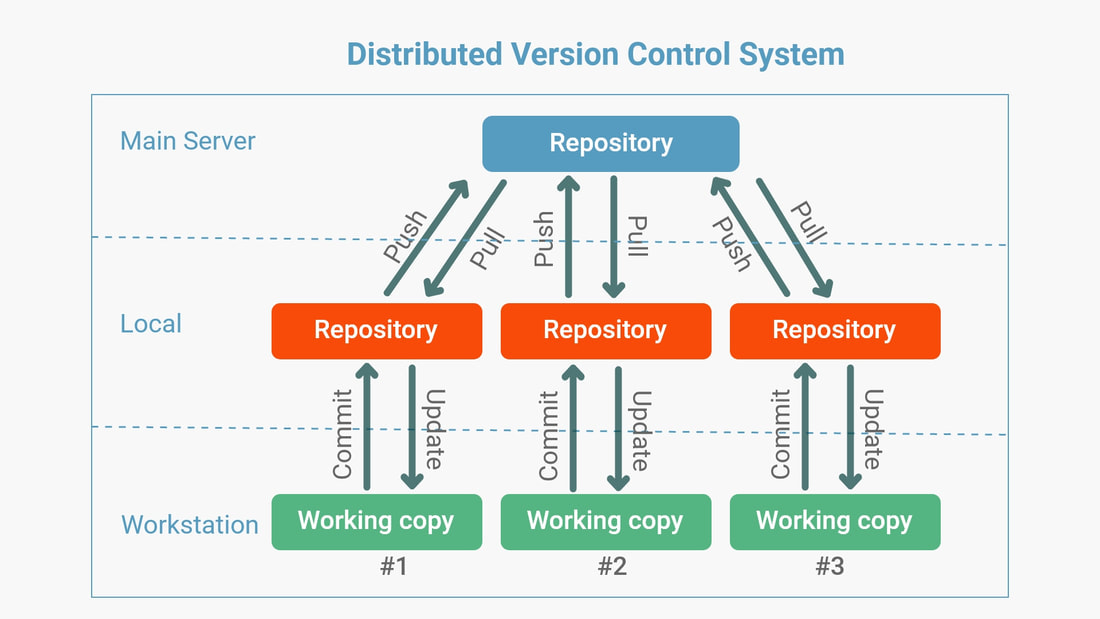
\includegraphics[width=0.85\textwidth]{distributed-vcs-structure}
    \caption{Distributed Version Control System (DVCS)}
    \label{fig:dvcs-structure}
\end{figure}

\subsubsection{Git}
\label{sec:git}
% Git is a distributed VCS that was developed by Linus Torvalds in 2005. Git is a free and open source VCS that is used by many large companies, such as Google, Facebook and Twitter. It is one of the most popular version control systems in use today.
% TODO: Rewrite this section
% ==============================================================================
Git was created in 2005 by Linus Torvalds (also the creator of Linux) and is written primarily in C combined with some shell scripts. It is widely considered the best VCS tool due to its features, flexibility, and speed. Linus Torvalds originally wrote it for the Linux codebase and it has grown to become the most popular VCS in use today.

"You can do a lot of things with Git, and many of the rules of what you should do are not so much technical limitations but are about what works well when working together with other people. So Git is a very powerful set of tools, and that can not only be overwhelming at first, it also means that you can often do the same (or similar) things different ways, and they all 'work.'" - Linus Torvalds

Git repositories are commonly hosted on local servers as well as cloud services. Git forms the backbone of a broad set of DevOps tools available from popular service providers including GitHub, BitBucket, GitLab, and many others.
\paragraph{Architecture}
Git is a distributed VCS. This means that no copy of the repository needs to be designated as the centralized copy - all copies are created equal. This is in stark contrast to the second generation VCS which rely on a centralized copy for users to checkin and checkout from.

What this means is that developers and coding partners can share changes with each other directly before merging their changes into an official branch. This allows team collaboration to take on a flexible distributed workflow, if desired.

Furthermore, developers can commit their changes to their local copy of the repository without any other repositories knowing about it. This means that commits can be made without any network or Internet connection. Developers can work locally offline until they are ready to share their work with others. At that point, the changes can be pushed to other repositories for review, testing, or deployment.

When a file is added for tracking with Git, it is compressed using the \lstinline{zlib} compression algorithm. The result is hashed using a SHA-1 hash function. This yields a unique hash value that corresponds specifically to the content in that file. Git stores this in an \lstinline{object database} which is located in the hidden \lstinline{.git/objects} folder.

The name of the file is the generated hash value, and the file contains the compressed content. These files are called Git blobs and are created each time a new file (or changed version of an existing file) are added to the repository.

"The object database is literally just a content-addressable collection of objects. All objects are named by their content, which is approximated by the SHA1 hash of the object itself. Objects may refer to other objects (by referencing their SHA1 hash), and so you can build up a hierarchy of objects." - Linus Torvalds

Git implements a \lstinline{staging index} which acts as an intermediate area for changes that are getting ready to be committed. As new changes are staged for commit, their compressed contents are referenced in a special index file - which takes the form of a \lstinline{tree} object. A \lstinline{tree} is a Git object that connects blob objects to their real file names, file permissions and links to other trees, and in this way represents the state of a particular set of files and directories. Once all related changes are staged for commit, the index tree can be committed to the repository, which creates a \lstinline{commit} object in the Git object database.

A commit references the head tree for a particular revision as well as the commit author, email address, date, and a descriptive commit message. Each commit also stores a reference to its parent commit(s) and so over time a history of project development is established.

As mentioned, all Git objects - blobs, trees, and commits - are compressed, hashed, and stored in the object database based on their hash value. These are called \lstinline{loose objects}. At this point no diffs have been utilized to save space which makes Git very fast since the full content of each file revision is accessible as a loose object.

However, certain operations such as pushing commits to a remote repository, storing too many objects, or manually running Git's garbage collection command can cause Git to repackage the objects into \lstinline{pack files}. In the packing process, reverse diffs are taken and compressed to eliminate redundant content and reduce size. This process results in \lstinline{.pack} files containing the object content, each with a corresponding \lstinline{.idx} (or index) file containing a reference of the packed objects and their locations in the pack file.

These pack files are transferred over the network when branches are pushed to or pulled from remote repositories. When pulling or fetching branches, the pack files are unpacked to create the loose objects in the object repository.

\paragraph{Basic Commands}

\begin{itemize}
    \item \lstinline{git init} - Initialize a Git repository in the current directory (creates the hidden \lstinline{.git} folder and its contents).
    \item \lstinline{git clone <git-url>} - Download a copy of the Git repository at the specified URL.
    \item \lstinline{git add <filename.ext>} - Add an untracked file or changed file to the staging area (creates corresponding entries in the object database).
    \item \lstinline{git commit -m 'Commit message'} - Commit a set of changed files and folders along with a descriptive commit message.
    \item \lstinline{git status} - Show information related to the state of the working directory, current branch, untracked files, modified files, etc.
    \item \lstinline{git branch <new-branch>} - Create a new branch based on the current checked-out branch.
    \item \lstinline{git checkout <branch>} - Checkout the specified branch into the working directory.
    \item \lstinline{git merge <branch>} - Merge the specified branch into the current branch checked-out in the working directory.
    \item \lstinline{git pull} - Update the working copy by merging in committed changes that exist in the remote repository but not the working copy.
    \item \lstinline{git push} - Pack loose objects for local active branch commits into pack files and transfer to remote repository.
    \item \lstinline{git log} - Show the commit history and associated descriptive messages for the active branch.
    \item \lstinline{git stash} - Save all uncommitted changes in the working directory to a cache so that they can be retrieved later.
\end{itemize}

% ==============================================================================
\subsubsection{Mercurial}
% Mercurial is a distributed VCS that was developed by Matt Mackall in 2005. Mercurial was developed with the same goal as Git, to maintain the Linux kernal project.
% TODO: Rewrite this section
% ==============================================================================
Mercurial was created in 2005 by Matt Mackall and it is written in Python. It was also started with the goal of hosting the codebase for Linux, but Git was chosen instead. It is the second most popular distributed VCS after Git, but is used far less often.
\paragraph{Architecture}
Like Git, Mercurial is a distributed version control system that allows any number of developers to work with their own copy of a project independently from others.

Mercurial leverages many of the same technologies as Git, such as compression and SHA-1 hashing, but does so in different ways.

When a new file is committed for tracking in Mercurial, a corresponding \lstinline{revlog} file is created for it in the hidden directory \lstinline{.hg/store/data/}. You can think of a \lstinline{revlog} (or revision log) file as a modernized version of the \lstinline{history files} used by the older VCS like CVS, RCS, and SCCS.

Unlike Git, which creates a new blob for every version of every staged file, Mercurial simply creates a new entry in the revlog for that file. To conserve space, each new entry only contains the delta (changes) from the previous version. Once a threshold number of deltas is reached, a full snapshot of the file is stored again.

This reduces the lookup time when applying many deltas to reconstruct a particular file revision.

These file revlogs are named to match the files that they track, but are postfixed with \lstinline{.i} and \lstinline{.d} extensions. The \lstinline{.d} files contained the compressed delta content. The \lstinline{.i} files are used as indexes to quickly track down different revisions inside the \lstinline{.d} files. For small files with low numbers of revisions, both the indexes and content are stored in \lstinline{.i} files. Revlog file entries are compressed for performance and hashed for identification. The hash values are referred to as \lstinline{nodeids}.

Whenever a new commit is made, Mercurial tracks the all file revisions in that commit in something called the \lstinline{manifest}. The manifest is also a revlog file - it stores entries that correspond to particular states of the repository.

However, instead of storing individual file content like the file revlogs, the manifest stores a list of filenames and nodeids that specify which file revision entries exist in each revision of the project. These manifest entries are also compressed and hashed. The hash values are again referred to as \lstinline{nodeids}.

Lastly, Mercurial uses one more type of revlog called a \lstinline{changelog}. The changelog contains a list of entries that associate each commit with the following information:
\begin{itemize}
    \item Manifest nodeid - Identifies the full set of file revisions that exist at a particular time.
    \item Parent commit nodeid(s) - This allows Mercurial to establish a timeline or branch of project history. One or two parent ID's are stored depending on the type of commit (normal vs merge).
    \item Commit author
    \item Commit date
\end{itemize}
Each changelog entry also generates a hash known as its \lstinline{nodeid}.

\paragraph{Basic Commands}
\begin{itemize}
    \item \lstinline{hg init} - Initialize the current directory as a Mercurial repository (creates the hidden \lstinline{.hg} folder and its contents).
    \item \lstinline{hg clone <hg-url>} - Download a copy of the Mercurial repository at the specified URL.
    \item \lstinline{hg add <filename.ext>} - Add a new file for revision tracking.
    \item \lstinline{hg commit -m 'Commit message'} - Commit a set of changed files and folders along with a descriptive commit message.
    \item \lstinline{hg status} - Show information related to the state of the working directory, untracked files, modified files, etc.
    \item \lstinline{hg update <revision>} - Checkout the specified branch into the working directory.
    \item \lstinline{hg merge <branch>} - Merge the specified branch into the current branch checked out in the working directory.
    \item \lstinline{hg pull} - Download new revisions from remote repository but don't merge them into the working directory.
    \item \lstinline{hg push} - Transfer new revisions to remote repository.
    \item \lstinline{hg log} - Show the commit history and associated descriptive messages for the active branch.
\end{itemize}

% ==============================================================================
\subsubsection{BitKeeper}
% TODO: Explain BitKeeper
\newpage
\newpage
% \subsubsection{Darcs Advanced Revision Control System (Darcs)}
% % TODO: Explain Darcs
\subsubsection{Monotone}
% TODO: Explain Monotone
\newpage
\newpage
\subsubsection{Bazaar}
% TODO: Explain Bazaar
\newpage
\newpage
\subsubsection{Fossil}
% TODO: Explain Fossil
\newpage
\newpage
% ==============================================================================
\section{Summary of Key Features}
\subsection{Repositories}
% TODO: Explain repositories
\subsection{Commits}
\newpage
% TODO: Explain commits
\subsection{Branching and Merging}
% TODO: Explain branching and merging
\newpage
\subsection{Pulling and Pushing}
% TODO: Explain pulling and pushing
\newpage
